\documentclass[12pt,american]{scrartcl}
\usepackage{babel}
\usepackage[babel]{microtype}
\usepackage[babel]{csquotes}
\usepackage[margin=0.75in]{geometry}

\usepackage[journal={Development},
			manuscript={DEVELOP/2023/201873},
			editor={Paul Francois}]{reviewresponse}

\usepackage[T1]{fontenc}
\usepackage{lmodern}
%\usepackage{newcent}
%\usepackage[scaled]{beramono}

\usepackage[backend=biber,style=ieee,dashed=false,url=false,isbn=false,defernumbers=true,refsection=section]{biblatex}
\bibliography{literature.bib}

\usepackage{hyperref}

\title{scTOP: physics-inspired order parameters for cellular identification and visualization}
\author{Maria Yampolskaya, Michael J Herriges, Laertis Ikonomou, Darrell N Kotton, and Pankaj Mehta}

\begin{document}
% \maketitle

% % Cover Letter
% Dear \editorname,


% Please find enclosed the revised version of our previous submission entitled \enquote{\thetitle} with manuscript number \manuscript. We would like to thank you and the reviewers for the valuable comments which help improving the quality of our manuscript.
% In this revision, we have carefully addressed the reviewers' comments. A summary of main modifications and a detailed point-by-point response to the comments from Reviewers 1 and 3 (following the reviewers' order in the decision letter) are given below.

\vspace{1.2em}

Sincerely,

\vspace{1.5em}

\theauthor

\vfil
\textbf{Note:} For clarity, each comment is displayed in a blue box, and additions to the manuscript are in gray boxes.

% Reviewer 1
\reviewer

\begin{revcomment}
	the important fact that the method is linear is mentioned but its implication is not really discussed. Many people will think that linear method = PCA (for instance), and it should be mentioned that the linear computation used is different from unsupervised linear methods such as PCA and SVD ( because of the reference set). Also the method could prove useful way beyond single cell data because of this (for instance many people use PCA for morphometrics analysis, and I could see how having a reference dataset to perform computation would help there).
\end{revcomment}
\begin{revresponse}
	We agree that this method is general enough to be applied to other contexts. We have added the following section to the Supplementary Information to explain how scTOP relates to other linear methods:
	\begin{changes}
		\subsection*{Comparison to other linear methods}
          scTOP is mathematically and conceptually distinct from other linear methods such as Principal Component Analysis (PCA). PCA takes input data and finds the vectors in feature space along which the most sample-to-sample variation occurs. PCA is unsupervised and assumes nothing is known about the input data. The principal components need to be examined to determine their biological relevance. The major difference with scTOP is that scTOP takes input data and a reference basis of known cell types. The input data is decomposed onto the vectors defined by the reference basis instead of vectors corresponding to the most sample-to-sample variation. With scTOP, the resulting decomposition has a direct interpretation: alignment with each of the known cell types within the reference basis. It’s not possible to find the decomposition onto known cell types with PCA, because PCA doesn’t have the extra information about pre-defined cell type expression profiles. 

          To summarize, scTOP and PCA both transform the sample data to a different coordinate system, but there are major differences between the spaces that these methods project onto. The following table breaks down the differences between these spaces.

          \begin{tabular}{ |p{2.5in}|p{2.5in}|} 
             \hline
             scTOP space & PCA space\\ 
             \hline
             \hline
             Defined by an input reference basis of known cell types & Calculated by PCA by finding the orthogonal vectors (principal components) that best explain the variation in data  \\ 
             \hline
             Can be non-orthogonal (e.g. can have highly-correlated cell types) & Orthogonal by definition  \\ 
             \hline
             Dimensions have clear biological interpretation: alignment with cell types & Dimensions need to be closely analyzed to be interpreted \\
             \hline
         \end{tabular}
	\end{changes}
\end{revresponse} \label{PCA}

\begin{revcomment}
	I see what the authors mean when they say it is important that the algorithms should give deterministic results, but in some cases, well controlled stochastic results could be necessary/important. I was thinking of MCMC based models, or similarly, instead of computing a deterministic order parameter, one could imagine algorithms giving meaningful probability scores while not being fully deterministic. In the end, the choice of the reference base certainly adds a quenched disorder component. Maybe the authors can elaborate a bit on this deterministic/stochastic issue because I suspect some people might not necessarily see the deterministic aspect as a strength 
\end{revcomment}
\begin{revresponse}
    We agree that stochastic results can be valuable. Rather than focus on the deterministic aspect of scTOP, we have edited the text to emphasize the importance of reproducibility rather than determinism. As you say, stochastic likelihood scores can also be useful; the important thing is the ability to make comparisons across analyses and data sets. We have changed the manuscript's mentions of determinism and stochasticity. For example, instead of ``Second, the algorithm should be deterministic, further enhancing reproducibility,'' the text now states:

    \begin{changes}
        Second, the results of the algorithm should be reproducible, so that direct comparison between data sets is possible.
    \end{changes}
\end{revresponse}

\begin{revcomment}
    the ‘mathematical details’ part is very condensed. It is certainly 
very readable for a physicist, but I do not think developmental 
biologists (even the ones interested in ‘modelling’) will be able to 
understand statements like ‘decorrelated versions of the conventional 
spin-glass magnetization’. I would recommend a short crash course for 
biologists on what an order parameter is, since it is the crucial 
concept to define scores. I like equations but I am not even sure they 
should be in the main text, I could for instance imagine a version of 
the paper where those concepts are explained in an intuitive/graphical 
way. At the very least more ‘intuitive’ details should be given to 
biologists.
\end{revcomment}
\begin{revresponse}
    As per the formatting guidelines for Development, we have moved the mathematical details to the ``Materials and Methods'' section after ``Discussion.'' We have also expanded the introduction section to give a more detailed explanation of what an order parameter is (the additions are in \textcolor{blue}{blue}).

    \begin{changes}
        Here, we present a new physics-inspired algorithm, single-cell Type Order Parameters (scTOP), that has all of these desired properties. The algorithm is based on the statistical physics concept of an order parameter -- a coarse-grained quantity that can distinguish between phases of matter. \textcolor{blue}{An order parameter takes on different values depending on the phase of the system. Typically, in a disordered phase, the corresponding order parameter is zero, and in an ordered phase it is nonzero.} Arguably the most famous example of an order parameter is magnetization in a ferromagnetic system, which is a collection of spins \textcolor{blue}{(in the simplest case, spins can be ``up'' or ``down'')} which align with one another. In a ferromagnet, the magnetization measures the alignment of spins and can be used to distinguish magnetic and paramagnetic phases. \textcolor{blue}{Below a particular temperature (known as the ``critical temperature''), the spins in the ferromagnet align with one another. In a simple model, the order parameter (magnetization, which measures the average spin) is approximately one if all the spins are up and approximately negative one if all the spins are down. When the temperature exceeds the critical temperature, the system changes from the magnetic phase to the paramagnetic phase, and the spins do not align; instead, they are randomly up or down, and the order parameter is approximately zero.}

        It is straightforward to generalize the idea of magnetization to more complex settings such as spin glasses and attractor neural networks. In the context of attractor-network epigenetic landscape models of cell identity, this takes the form of generalized magnetizations that measure how aligned a gene expression state is with each of the attractor basins for different cell fates. \textcolor{blue}{Whereas magnetization for the ferromagnetic system measured whether the system was in a magnetic or paramagnetic phase, these generalized magnetizations measure which phase a gene regulatory network is in (where the different phases correspond to different cell types).} These generalized magnetizations serve as natural order parameters for cellular identity and can be calculated directly from data. The scTOP algorithm builds on previous work by developing methods for integrating scRNA-seq data, greatly expanding the power and utility of this approach. 
    \end{changes}
\end{revresponse}

\begin{revcomment}
    in physics magnetization and spins could range from -1 to +1, here the
 order parameter is always positive (and lower than 1) as far as I can 
see. why ? In particular it is not entirely clear to me how things were 
put back between 0 and 1. Also, the maximum value of the order parameter
 computed from data seems to be around 0.5, can the authors comment on 
the magnitudes computed by their algorithm and how to interpet them ?
\end{revcomment}
\begin{revresponse}
    scRNA-seq data is very sparse, so it’s not possible to reach perfect alignment (score of +1). The reference basis contains aggregate profiles, where expressions have been averaged across cells of the same type. This removes many of the zeroes, but the single-cell samples still have many zeroes, resulting in misalignment. When samples are averaged in order to find aggregate scores, it’s possible to reach higher scores thanks to the reduction in zeroes. The figure with the aggregate samples from the Mouse Cell Atlas compared to organs from Tabula Muris illustrates these higher scores. It also shows a few scores that are negative.
    
    We have also added the following section to the Supplementary Information:
    \begin{changes}
        \subsection*{Interpreting scTOP scores}
        In theory, the attractor-network order parameters we have adapted for gene expression data range between negative one and positive one. An attractor state order parameter with a value of positive one means the system is perfectly aligned with that particular attractor state, and negative one means it is the exact opposite of that attractor state. Zero means that it is neither correlated nor anti-correlated with that attractor state. 
        
        In practice, scTOP scores generally do not reach positive one. scRNA-seq data contains significant numbers of dropouts, and these zeroes decrease the magnitude of the scTOP score. When an aggregate score is taken, the effect of dropouts is decreased and the scTOP score increases. This is important to keep in mind when interpreting scTOP scores; any score above 0.1 is notable, and since the data is so noisy even the best-case score may be well below 1. It's helpful to have a control population to compare with, to have a measure of the range of best-case scTOP scores. This is also why it's best to compare distributions of scores rather than scores for individual cells, since noise plays a non-negligible role.
        
        scTOP scores are rarely negative. Negative values for scTOP scores correspond to cases where the sample gene expression profile is the opposite of the reference profile. For example, a score of -1 would indicate that all the genes which are highly-expressed in the reference are lowly-expressed in the sample, and vice versa. There are cases where the scores are low, negative values, indicating that the sample does not align well with the reference and that some genes which are highly- (lowly-) expressed in the reference are lowly- (highly-) expressed in the sample. From the data, it appears that it’s unlikely for gene networks to contain cell types which are opposites of one another. One possible reason is that some genes, like housekeeping genes, are similarly expressed across all cell types. Also, it’s possible that cells which expressed the exact opposite genes of any given cell type would not be able to survive.
    \end{changes}
\end{revresponse}

\begin{revcomment}
    when commenting on $S^\perp$, it is qualified as ‘biological noise’, but
 then reference to cell cycle genes, etc… is made. I can imagine genes 
related to, say, oscillating genes in the segmentation clocks, which 
would definitely be thrown away by the method (because they do not 
correspond to actual cell fates) but are definitely not developmental 
noise either. Maybe some comment should be added on situations like 
this, where gene dynamics not clearly associated with ‘fates’ (as 
defined by humans in their reference dataset) can not really be 
detected/visualized with this method. Along the same lines, it could be 
useful to show what happens with ‘virtual’ experiments where some 
reference fates are removed to contrast them with the situation with all fates
\end{revcomment}
\begin{revresponse}
    We agree that one of the limitations of scTOP is that it gives only information on cell differentiation. It cannot capture the dynamics of gene expression beyond the changing of alignment with cell identities defined by the reference basis. To clarify this point, we have edited the $S^{\perp}$ paragraph:

    \begin{changes}
        Biologically, $S^{\perp}$ contains information about processes that affect gene expression but are not associated with cell identity, such as the cell cycle. We refer to the $a^{\mu}$ as the scTOP scores. Each component of this vector measures the projection of the cell with gene expression profile $S_i$ onto the $\mu$ - the cell type in the reference basis. These scores can be used to accurately classify cell identity and provide a natural visualization of gene expression in the space of possible cell fates. Gene regulatory dynamics that are unrelated to transitions between cell types in the reference basis would not be captured by these scores; instead, these would contribute to $S^{\perp}$. As a result, these fate-unrelated dynamics cannot be visualized using scTOP.
    \end{changes}
\end{revresponse}

\begin{revcomment}
The authors only show ‘2D’ representation, for two order parameters. 
Is this because they only see binary choices in the data? Could we see 
in 3D a sequence of two binary choices for instance ? Is there anything 
biological to tell there?
\end{revcomment}
\begin{revresponse}
    It can be difficult to distinguish the positions of points in a 3D scatter plot. We have included figure \ref{3D plots} here to illustrate this. In this figure, we plot a clonal family from the hematopoietic data set in the main text. This is a case where multiple cell identities are of interest, but it is difficult to discern their relationships from a 3D plot. In cases where multiple fates are of interest, in binary choices or otherwise, we use pair-plots to show multiple 2D projections simultaneously.

    \begin{figure}
	\centering
    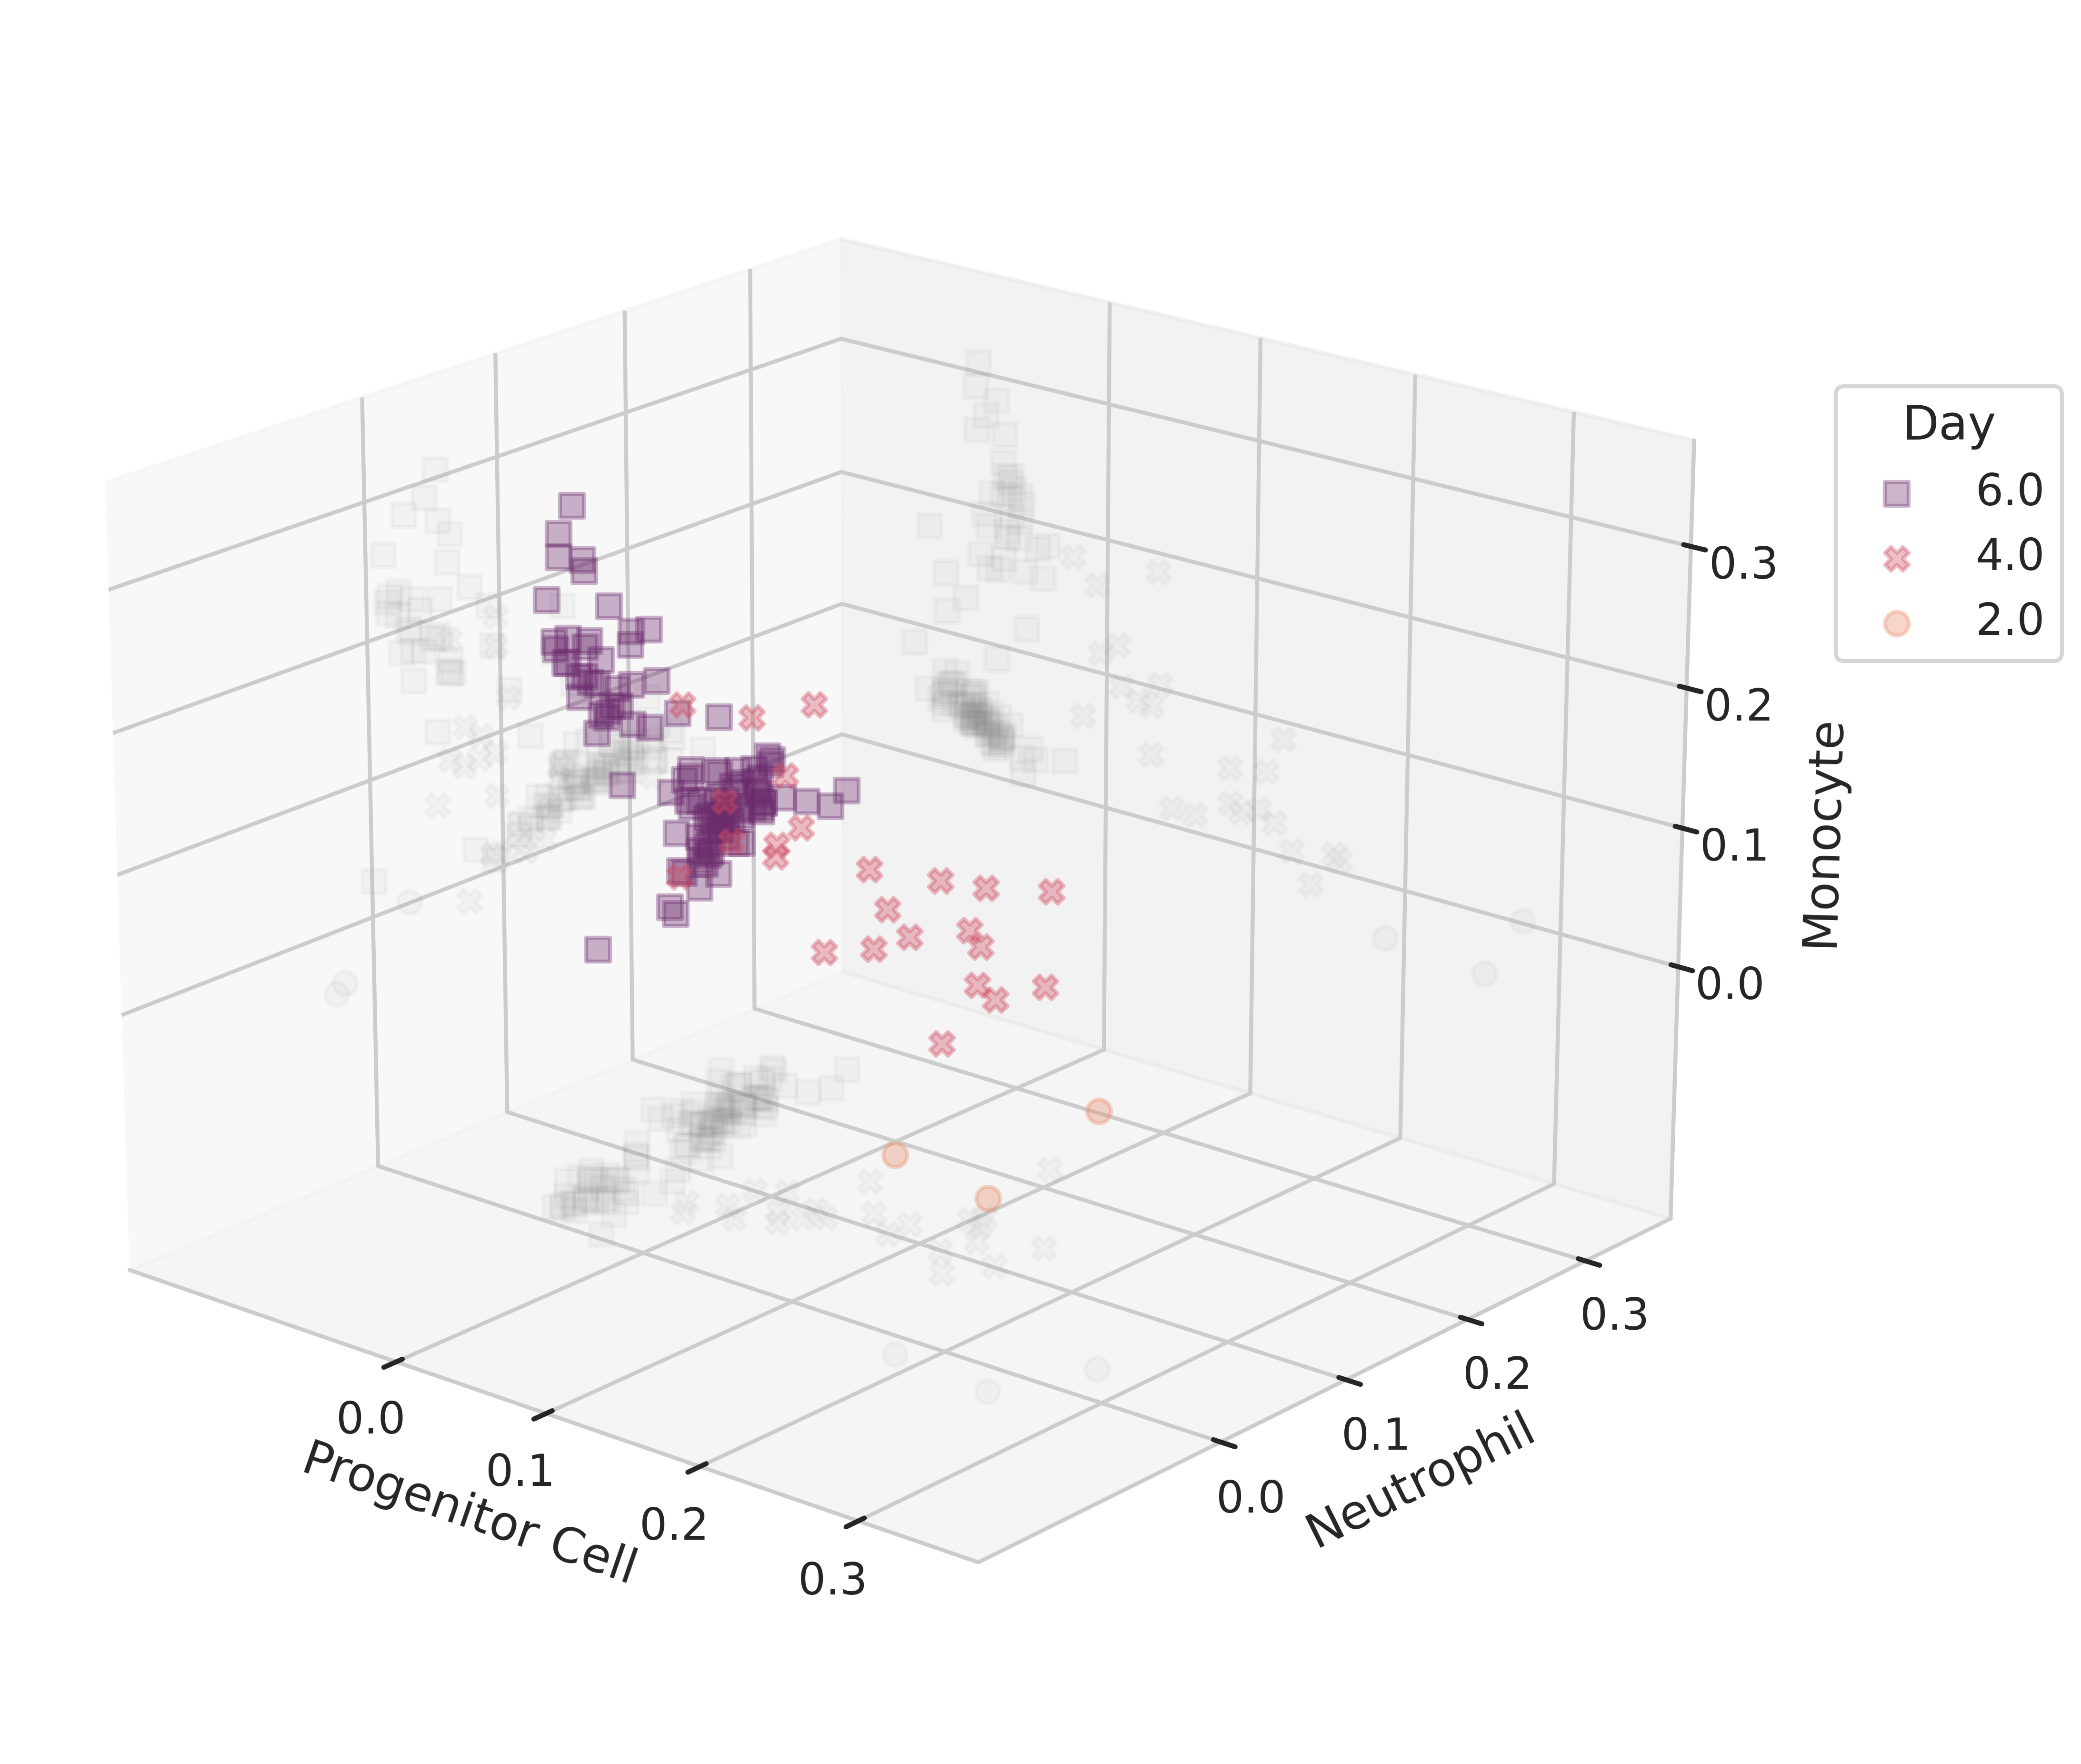
\includegraphics[scale=0.3]{figs/hem 3d neutrophil-monocyte.png}
	\caption{An example of a three-dimensional representation of scTOP scores, in the case of hematopoietic differentiation. Even with the inclusion of "shadows" (the corresponding 2D projections on the boundaries) it is difficult to determine the relationships between cells, which is why we use pair-plots in the main text instead. }
	\label{3D plots}
    \end{figure}
\end{revresponse}

\begin{revcomment}
    Table I : it is a bit unclear to me how the method was validated when 
Query data are used on the same reference set. I was expecting something
 classic like an initial separation between training/validating 
ensembles, etc… But it rather seems from the Supplement that the 
training set essentially was based on ‘well-chosen’ cells or something 
like this. It could be useful to give more details in the main text.
\end{revcomment}
\begin{revresponse}
    We do have the initial separation between training and test data. For clarity, we have changed the table column names to ``Test data source'' and ``Reference data source,'' and we have added the following line to the main text:
    \begin{changes}
        For cases where the training (or ``reference'') data source is the same as the test data source, we set aside a randomly-selected subset of cells for the training set and do not use them in the test data.
    \end{changes}

    The discussion of curating data sets in the SI refers to the cell types, rather than the cells, that were chosen for the reference basis. In other words, we discard cell types that have fewer than 100 corresponding cells. We do this because scRNA-seq data has a lot of dropouts, so we need to average across many cells to get a reasonable reference basis. We want to make sure the reference gene expression profiles are reflective of the true gene expression profiles of the cell types; making sure there are enough training data points per cell type is what we mean by having "well-sampled" reference profiles.

    To demonstrate the effect of not having enough cells per cell type, we have included figure \ref{sampling}. In this figure, we vary the number of cells sampled for the reference cell type profile, and find the corresponding scTOP score for the query data. With very few cells, the score is low since the reference type is poorly sampled. As the number of cells increase, the score plateaus. Ideally, we would have thousands of cells for every cell type, but unfortunately many single-cell data sets do not have so many cells per cell type.

    \begin{figure}
	\centering
    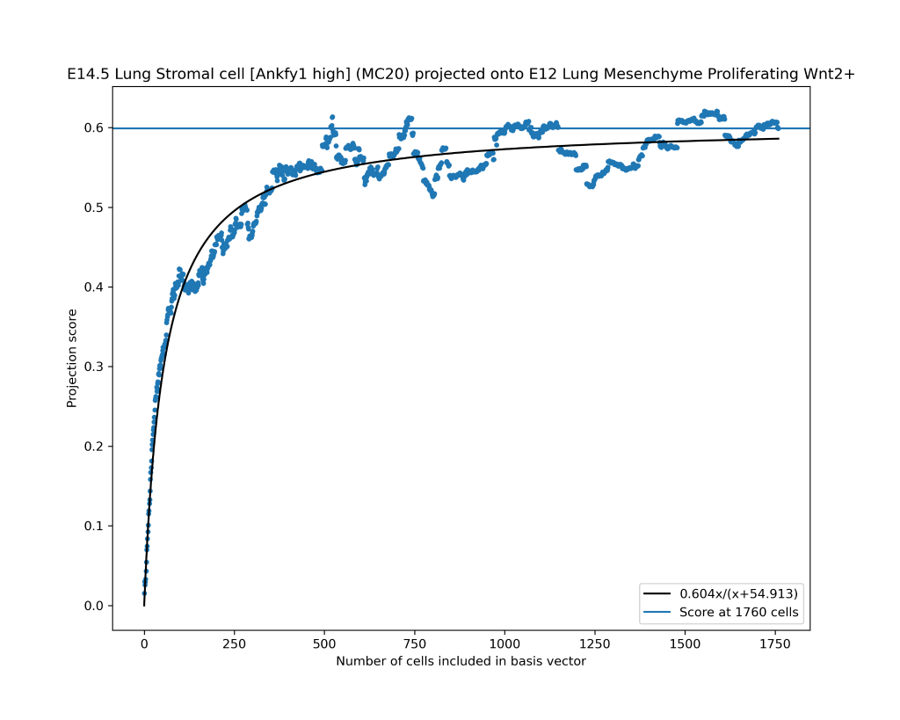
\includegraphics[scale=0.4]{figs/sampling.png}
	\caption{A plot of adult mouse lung stromal cells from the Mouse Cell Atlas projected onto a reference profile calculated from mesenchymal cells from the Atlas of Lung Development \cite{negretti2021single}. The x-axis indicates the number of cells sampled for the reference cell type, and the y-axis indicates the scTOP score. }
	\label{sampling}
    \end{figure}
\end{revresponse}

\begin{revcomment}
along the same line, all results depend on the quality of the 
reference set. Is there a way to somehow benchmark it ? For instance, I 
could imagine that a bad reference set could give a lot of false 
negatives or false positives, how would we see this ? (maybe by 
comparing with some unsupervised method ?)
\end{revcomment}
\begin{revresponse}
    In order to benchmark the quality of the reference bases, we measured the accuracy scores of control samples scored with those bases. In the manuscript, we provide examples of comparing the accuracy metrics with unsupervised methods from Abdelaal et al. In particular we compare the F1 score for scTOP using the CellBench and Allen Mouse Brain atlas with the F1 scores achieved for the same data sets using a variety of automatic cell identification algorithms, including unsupervised methods. The F1 score is a metric that is calculated from the true positives, false positives, and false negatives. 

    Similar algorithms are often black boxes that are difficult to troubleshoot, but since scTOP simply uses linear algebra, it is possible to determine which genes are contributing to the scTOP scores. If a reference basis is giving a dubious result, it's possible to check if the top-contributing genes correspond to relevant biological processes. If not, this indicates that the reference basis may be poorly constructed, whether due to not having enough cells per cell type or not having distinct enough cell types.
\end{revresponse}

\begin{revcomment}
    The paper reads a bit long to me (12 figures, please check ). Maybe 
some figures with very similar messages/methods could be combined (e.g. 
4,5,6) and the writing could be a bit tightened there as well. There is a
 lot of ‘empty space’ in some figures (eg 9, 12) which could be 
tightened
\end{revcomment}
\begin{revresponse}
    In addition to ensuring that all figures match the formatting guidelines, we have made the following changes:
    \begin{enumerate}
        \item We have adjusted the layout and removed whitespace from figures 1, 5, and 6
        \item We have removed redundant panels (or moved them to the Supplementary Information), as in figures 5 and 9
        \item We have moved figure 8 to the Supplementary Information
        \item We have combined three figures into the panels of figure 4, and tightened the writing accordingly
    \end{enumerate}
\end{revresponse}

\begin{revcomment}
    1st sentence : « humans and other mammals… » I guess other animals too
\end{revcomment}
\begin{revresponse}
    We have fixed this line to say "humans and other animals."
\end{revresponse}

% Reviewer 2
\reviewer

\begin{revcomment}
	What is the relationship of scTOP to PCA? Presumably one could do PCA with C principal components for C distinct cell types and construct a new coordinate system as the average vector to each celltype. How should one think about this wrt to scTOP’s basis vectors? Can you perhaps provide a comparison of how the two methods fair when thinking about cell types or intermediates and even lineages
\end{revcomment}
\begin{revresponse}
 Although scTOP and PCA are both linear methods, there are significant differences between them. The principal components computed by PCA are the orthogonal dimensions that describe the most variance in the data. For example, the first principal component is the dimension along which the data varies the most. Taking C principal components would not provide information about alignment to the C cell types; instead, this coordinate system would give information about the top C dimensions along which there is the most variance. For example, if the input data corresponded to cells that were all of cell type A, the principal components would give information about how the gene expression varies between these cells, regardless of cell type. On the other hand, scTOP would identify all these cells as cell type A.

 We have added the following section to the Supplementary Information to explain how scTOP relates to other linear methods:
	\begin{changes}
		\subsection*{Comparison to other linear methods}
          scTOP is mathematically and conceptually distinct from other linear methods such as Principal Component Analysis (PCA). PCA takes input data and finds the vectors in feature space along which the most sample-to-sample variation occurs. PCA is unsupervised and assumes nothing is known about the input data. The principal components need to be examined to determine their biological relevance. The major difference with scTOP is that scTOP takes input data and a reference basis of known cell types. The input data is decomposed onto the vectors defined by the reference basis instead of vectors corresponding to the most sample-to-sample variation. With scTOP, the resulting decomposition has a direct interpretation: alignment with each of the known cell types within the reference basis. It’s not possible to find the decomposition onto known cell types with PCA, because PCA doesn’t have the extra information about pre-defined cell type expression profiles. 

          To summarize, scTOP and PCA both transform the sample data to a different coordinate system, but there are major differences between the spaces that these methods project onto. The following table breaks down the differences between these spaces.

          \begin{tabular}{ |p{2.5in}|p{2.5in}|} 
             \hline
             scTOP space & PCA space\\ 
             \hline
             \hline
             Defined by an input reference basis of known cell types & Calculated by PCA by finding the orthogonal vectors (principal components) that best explain the variation in data  \\ 
             \hline
             Can be non-orthogonal (e.g. can have highly-correlated cell types) & Orthogonal by definition  \\ 
             \hline
             Dimensions have clear biological interpretation: alignment with cell types & Dimensions need to be closely analyzed to be interpreted \\
             \hline
         \end{tabular}
	\end{changes}
\end{revresponse}

\begin{revcomment}
    The authors say scTOP does not require data harmonization and 
is able to distinguish between technical and biological noise, but 
couldn’t batch effects between the reference dataset and the sample 
dataset effect the results? Can you use some dataset to illustrate this,
 there are few discussed in the several batch correction papers?
\end{revcomment}
\begin{revresponse}
    scTOP is able to identify cell types and give similar score distributions even across data sets. To demonstrate this, we analyzed dataset 4 from Tran et al. \cite{tran2020benchmark}. This data set contains pancreatic data from 5 different sources. We have added the following section to the Supplementary Information:

    \begin{changes}      
        \subsection*{Batch effects}
        scRNA-seq data produced using different sequencing platforms from different experiments may introduce variation in the form of batch effects. Because the pre-processing step in scTOP prioritizes the relative rather than absolute expression of genes, batch effects are mitigated.
        
        Tran et al. \cite{tran2020benchmark} consolidated datasets from different experiments for the purposes of benchmarking various batch-effect correction methods. One of these is a dataset containing scRNA-seq human pancreatic data from five different sources \cite{baron2016single} \cite{muraro2016single} \cite{segerstolpe2016single} \cite{wang2016single} \cite{xin2016rna}, using various sequencing technologies. We used scTOP to analyze these datasets. Figure \ref{batch effects} illustrates that scTOP is not significantly affected by differences between batches. Because the Baron et al. dataset had the most cells per cell type, we used it to create a reference basis consisting of alpha, beta, ductal, acinar, delta, gamma, stellate, and endothelial gene expression profiles. We projected cells from the other four experiments onto the Baron reference basis. The top row shows kernel density estimate (KDE) plots for cells that match the reference cell type (e.g. alpha scores for alpha cells) with solid lines, and cells that do not match the reference type but have higher scores than the other non-matching types (e.g. alpha scores for beta cells) with dashed lines. The bottom row shows box-and-whisker plots for the cells that match the reference type.

        Despite coming from different sources, the distributions of scores are similar. There is also a clear bimodal distribution for cells that match the reference type and cells that don't. This bimodality is a clear indication that batch effects don't cause misidentification.
        
        According to Ziegenhain et al. \cite{ziegenhain2017comparative}, Smart-seq2 detects the most genes per cell when compared to other sequencing methods of that time. This decrease in dropouts may explain why the Segerstolpe data (which is the only experiment that used Smart-seq2) has slightly higher projections than the other datasets.
    \end{changes}

    \begin{figure}
	\centering
    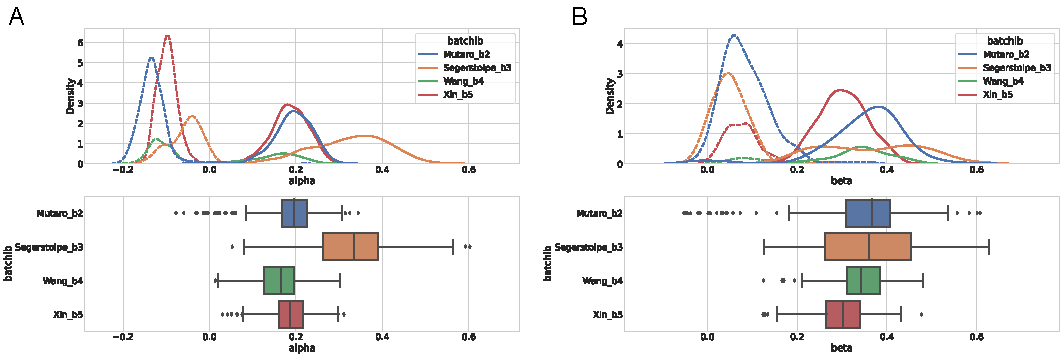
\includegraphics[scale=0.95]{figs/batch effects.pdf}
	\caption{Pancreatic data from different experiments using different scRNA-seq technologies. The reference basis uses data from Baron et al. \cite{baron2016single}, and the cells that are projected onto this basis are from Muraro et al. \cite{muraro2016single}, Segerstolpe et al. \cite{segerstolpe2016single}, Wang et al. \cite{wang2016single}, and Xin et al. \cite{xin2016rna} (A) Kernel density estimate (KDE) plot of alpha scTOP scores for alpha cells (solid) and beta cells (dashed), and a box-and-whisker plot of alpha scTOP scores for alpha cells. (B) KDE plot of beta scTOP scores for beta cells (solid) and delta cells (dashed), and a box-and-whisker plot of beta scTOP scores for beta cells. }
	\label{batch effects}
    \end{figure}
\end{revresponse}

\begin{revcomment}
    Authors mention that pre-processing to generate z-scores is essential.
 It is not clear why that should be, at least authors don’t explain it. 
For example, does a simpler, more intuitive normalization per cell of 
converting counts to fractions, work? I think there are many schemes of 
normalizations that have been proposed and having a clear analysis and 
discussion around that is essential for “users” who may be interested in
 using scTOP.
\end{revcomment}
\begin{revresponse}
    To address this comment, we have added the following subsection under the ``Preprocessing'' section of the Supplementary Information.

    \begin{changes}
    \subsection*{Preprocessing rationale} 

    In order to mitigate batch effects, the preprocessing step in scTOP takes each cell and ranks each gene according to expression. These ranks are converted into percentiles, which are then transformed into z-scores assuming a normal distribution.
        
    By ranking the genes before converting to z-scores, we are ignoring the absolute values of RNA counts and instead focusing on the relative values. Some sequencing platforms may measure many more counts than others; although we can't recover the unmeasured counts that are lost via dropouts, we can remove the effect of differences in counts by ranking. We assume that each cell contains similar numbers of mRNA and that the actual number of RNA doesn't matter as much as the relative expression of different genes. For example, the highest-expressed gene in one cell should be comparable to the highest-expressed gene in another cell, regardless of RNA count. Ignoring the absolute values of RNA counts reduces the differences caused by different scRNA-seq technologies and experiments, as shown by the ``Batch effects'' section.
    
    The second preprocessing step is to convert the ranks to z-scores, assuming a normal distribution. This step results in a mean of zero and standard deviation of one. In data analysis, it is beneficial to standardize the data before comparing across datasets because this prevents a disproportionate bias towards features with large values. In the case of scTOP, having a mean of zero and a standard deviation of one is especially important because the underlying math relies on the dot product of two uncorrelated vectors to be zero and the magnitude of a vector to be one.
    
    By ranking and z-scoring, we remove undue weighting of genes according to magnitude of expression, instead prioritizing the relative expression.
    \end{changes}
    
\end{revresponse}

\begin{revcomment}
    About lineages, this is perhaps the most important application of 
scTOP as it brings out something beyond cell types that was the input to
 the system. The authors have some discussion of how having fewer cell 
types make it harder to map out the space and hence the lineages. But 
many applications where one is interested in cell fate dynamics of only a
 handful of cell types, sometimes one cell type going to two, is central
 to understand the underlying genetic logic of that drives the cascade 
of “bifurcations”. This feels like a big limitation, and I am curious if
 authors to say a little more on this, perhaps again by taking a 
concrete example, either with synthetic or real data.
\end{revcomment}
\begin{revresponse}
    One limitation of scTOP is that a certain number of cells are needed per cell type in order to create an accurate expression profile for that cell type. While having more cell types can indeed help map out the cell type subspace, most cell types can be removed from the reference basis and scTOP scores are still able to distinguish the remaining types (see Supplementary Information section ''Robustness of scTOP``, which shows the result of having few cell types in the reference basis). 

    scTOP is able to visualize the cell fate dynamics of one cell type going to two. A concrete example can be found in the hematopoiesis lineage tracing data. In this dataset, clonal families with three time points reveal the dynamics of hematopoietic stem cells differentiating into mature blood cells. Figure 6 shows the scTOP scores of individual clonal families (i.e. sister cells that originated from the same stem cell) over time. One of these plots shows the case of one cell type going to two: progenitor cells going to neutrophil and monocytes. The plot with basophils, neutrophils, and eosinophils shows one cell type going to three other cell types. Another example of one cell type going to two is shown by the AT1/AT2 plots, where a lung alveolar progenitor cell differentiates into either AT1 or AT2.

    The biggest limitation of scTOP is the case where the cell type of a sample of interest is not included in the reference basis. In this case, all the corresponding scTOP scores will be low, unless the cell type of the sample is highly correlated with a cell type in the basis. For this reason, the scTOP scores may be sensitive to change when highly-correlated cell types are added or removed.
\end{revresponse}

\begin{revcomment}
    Also, on lineages, could some analysis be provided to see if expected gene expression changes happen along the directions of cell fate changes? This would provide some confidence on the predicted cell fate 
dynamics.
\end{revcomment}
\begin{revresponse}
    Figure 5 of the main text shows the development of mouse alveolar cells. The scTOP scores for AT1 and AT2 are shown for each time point of this time series data, and each cell is colored by the expression of AT1 or AT2 marker genes. These marker genes are the genes that are expected to change and become highly expressed when AT1 or AT2 fates are adopted. As shown by the plots, expression of these marker genes occurs along the directions of cell fate indicated by scTOP. The expected gene expression changes do occur with the dynamics visualized by scTOP.
\end{revresponse}

\begin{revcomment}
    You should explicitly mention “xi” is the basis in methods 
section II A. I don’t think its explicitly mentioned anywhere and would 
be useful for readers not familiar with these types of methods.
\end{revcomment}
\begin{revresponse}
    To address this comment, we have added the following line:

    \begin{changes}
         We refer to $\xi$ as the reference basis.
    \end{changes}
\end{revresponse}

\begin{revcomment}
    Figure 2 a,b,c are referred to in the text but the figure does not contain these labels.
\end{revcomment}
\begin{revresponse}
    To address this comment, we have edited the figure and added labels.
\end{revresponse}

\begin{revcomment}
    What is the interpretation of a negative scTOP score? Some of the plots contain small negative values. For example, in Figure 2 when plotting Ciliated vs AT2, cells high along the Ciliated axis become increasingly negative along the AT2 axis. Are these cells more or less like AT2 cells than the zero point? A similar result is seen in Figure 7 where high AT1 axis cells become increasing negative along the AT2 axis. Some other moderately high negative values are also seen in Figure 4 and 6.
\end{revcomment}
\begin{revresponse}
    To address the interpretation of negative scores, we have added the following section to the Supplementary Information:
    \begin{changes}
        \subsection*{Interpreting scTOP scores}
        In theory, the attractor-network order parameters we have adapted for gene expression data range between negative one and positive one. An attractor state order parameter with a value of positive one means the system is perfectly aligned with that particular attractor state, and negative one means it is the exact opposite of that attractor state. Zero means that it is neither correlated nor anti-correlated with that attractor state. 
        
        In practice, scTOP scores generally do not reach positive one. scRNA-seq data contains significant numbers of dropouts, and these zeroes decrease the magnitude of the scTOP score. When an aggregate score is taken, the effect of dropouts is decreased and the scTOP score increases. This is important to keep in mind when interpreting scTOP scores; any score above 0.1 is notable, and since the data is so noisy even the best-case score may be well below 1. It's helpful to have a control population to compare with, to have a measure of the range of best-case scTOP scores. This is also why it's best to compare distributions of scores rather than scores for individual cells, since noise plays a non-negligible role.
        
        scTOP scores are rarely negative. Negative values for scTOP scores correspond to cases where the sample gene expression profile is the opposite of the reference profile. For example, a score of -1 would indicate that all the genes which are highly-expressed in the reference are lowly-expressed in the sample, and vice versa. There are cases where the scores are low, negative values, indicating that the sample does not align well with the reference and that some genes which are highly- (lowly-) expressed in the reference are lowly- (highly-) expressed in the sample. From the data, it appears that it’s unlikely for gene networks to contain cell types which are opposites of one another. One possible reason is that some genes, like housekeeping genes, are similarly expressed across all cell types. Also, it’s possible that cells which expressed the exact opposite genes of any given cell type would not be able to survive.
    \end{changes}
\end{revresponse}

\begin{revcomment}
    Are there any dataset-specific preprocessing steps done? For example filtering cells or genes based on quality control metrics. If so, they 
should be reported so that the results are reproducible.
\end{revcomment}
\begin{revresponse}
    We took the datasets as they were deposited and did not filter any genes. As described in the Supplementary Information section ``Reference basis construction,'' we discarded cells if there were fewer than 100 cells of the corresponding cell type. This is because the reference basis needs at least 100 cells per cell type in order to represent accurate expression profiles for the given cell types.
\end{revresponse}

\begin{revcomment}
    The code in the linked Github repository contains a tutorial, but the
 code used to run scTOP on the other datasets should also be provided.
\end{revcomment}
\begin{revresponse}
    We have made the following changes to address this comment:

    \begin{changes}
        We have implemented scTOP in an easy-to-use Python package, available on the \href{https://pypi.org/project/scTOP/}{Python Package Index} and \href{https://github.com/Emergent-Behaviors-in-Biology/scTOP}{Github}. The code for the analyses in this paper is available in a separate \href{https://github.com/Emergent-Behaviors-in-Biology/scTOP-manuscript}{Github repository}.
    \end{changes}
\end{revresponse}

\printbibliography

\end{document}